\chapter{Capa de Motivación}
\section{Introducción}

Esta capa retoma, en primer lugar, algunos de los conceptos utilizados en la capa de negocio como por ejemplo el concepto de rol representado en esta capa como un Interesado (StakeHolder) y el concepto de servicio el cual tiene como equivalente un Objetivo(Goal)\cite{BolanosCastro2019}.

Es importante entender el uso e interacción de los elementos que definen la estructura de la organización, durante el proceso de apropiación de conceptos que se presenta en esta capa, se destacan los diferentes aspectos motivacionales que denotan principalmente aspectos organizacionales, en términos de cada una de las entidades encontradas y sus interacciones. Entidades como objetivos y principios que
determinan de forma detallada aspectos fundamentales de la estructura organizacional (objetivos, plan estratégico, misión y visión)\cite{BolanosCastro2019}.

Por otra parte, es importante resaltar que, dentro de la estructura organizacional un aspecto clave corresponde a las relaciones que se presentan entre los diferentes elementos. A nivel externo (principios, interesados) e interno (objetivos, requerimientos) de la organización se pueden ver estas interacciones que representan los diferentes servicios ofrecidos, mencionando sus detalles a través de requerimientos y restricciones, y también los diferentes roles que interactúan en este escenario (interesados, manejador)determinando así la comunicación entre los conceptos organizacionales \cite{BolanosCastro2019}. 

A continuación se presentan cada uno de los puntos de vista de la capa de Motivación  a partir del soporte realizado por el Área de Investigación de Análisis de datos a los investigadores de la Subdirección de Investigaciones, otras Subdirecciones y demás unidades funcionales del Instituto de Cancerología.

%-------------Punto de Vista de la Infraestructura----------%
\newpage
\section{Punto de Vista de Interesados}
El Punto de Vista de Interesados permite al analista modelar las partes interesadas, los impulsores internos y externos del cambio y las evaluaciones en términos de fortalezas, debilidades, oportunidades y amenazas de dichos controladores . Ademas,se pueden describir los vínculos con los objetivos iniciales de alto nivel que abordan estas preocupaciones y evaluaciones. Estos objetivos forman la base para el proceso de ingeniería de requisitos, incluyendo refinamiento de objetivos, contribucion y análisis de conflictos, y la derivación de requisitos que realicen las metas\cite{BolanosCastro2019}.

En la Figura \ref{PvInteresados}, se plantea el Caso para el Punto de Vista de Interesados con cada uno de los elementos que interactúan entre sí. 

\begin{figure}[h!]
	\centering
	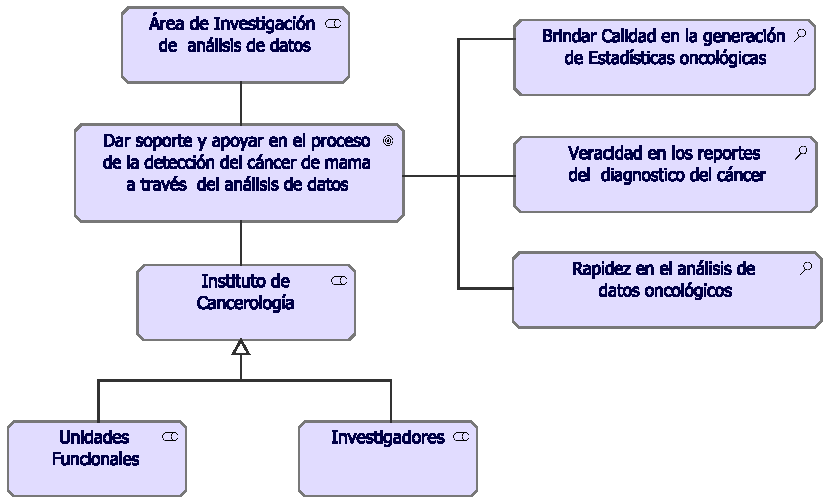
\includegraphics[width=1\linewidth]{ARQUITECTURA/imgs/CapaMotivacion/1_PvInteresados}
	\caption{Punto de Vista de Interesados}
	\label{PvInteresados}
\end{figure}

\begin{enumerate}[label=\textbf{\arabic*})]
	

\item  \textbf{Área de Investigación de análisis de datos:} Corresponde a una de las dependencias del área de investigación la cual  tiene por objetivo dar soporte a los investigadores de la Subdirección de Investigaciones, otras Subdirecciones y demás unidades funcionales del Instituto de Cancerología, haciendo uso métodos computacionales para el manejo y análisis de datos Oncológicos.
	
\item  \textbf{Dar soporte y apoyar en el proceso de la detección del cáncer de mama a través del análisis de datos:} Este objetivo organizacional hace referencia a el servicio de generar diagnósticos relacionados con el cáncer de mama  solicitados por los diferentes funcionarios del Instituto de Cancerología.Se asocia con dos Stakeholder: \textit{Área de Investigación de análisis de datos} e \textit{Instituto de Cancerología}; el primero es el que vela por el cumplimiento del objetivo;el segundo es a quien se brinda el servicio del Diagnostico del Cáncer de mama. 

\item  \textbf{Instituto de Cancerología:} Este rol de aplicación corresponde a los diferentes usuarios del instituto de nacional de cancerología. Tienes asociado el actor \textit{Investigadores} y el actor \textit{Unidades funcionales }. Estos roles se describen a continuación: 
\begin{itemize}
	\item  \textbf{\textit{Investigadores:}}  Este rol está conformado por todos los grupos de investigación en cáncer del país registrados ante Colciencias y adicionalmente, con representantes de diferentes tipos de usuarios del conocimiento generado por la investigación como son las sociedades médicas, los prestadores de servicios oncológicos, los aseguradores, las autoridades sanitarias y los pacientes entre otros. 
	
	\item  \textbf{\textit{Unidades Funcionales :}}  Este rol está conformado por las unidades clínicas ubicadas al interior del Instituto de Cancerología cuya función es evaluar la situación de salud del paciente con diagnóstico presuntivo de cáncer. 
\end{itemize}

\item  \textbf{Brindar Calidad en la generación de Estadísticas Oncológicas:} Teniendo en cuenta el objetivo \textit{Dar soporte y apoyar en el proceso de la detección del cáncer de mama a través del análisis de datos}, se tiene esta valoración. En este caso, el resultado es la oportunidad de generar calidad en la información estadística acerca de la identificación del cáncer de mama diversos pacientes.

\item  \textbf{Veracidad en los reportes del diagnostico:} Teniendo en cuenta el objetivo \textit{Dar soporte y apoyar en el proceso de la detección del cáncer de mama a través del análisis de datos}, se tiene esta valoración. En este caso, el resultado es la oportunidad de generar diagnósticos exactos acerca de las posibilidad de padecer cáncer de mama.  

\item  \textbf{Rapidez en el análisis de datos oncológicos:} Teniendo en cuenta el objetivo \textit{Dar soporte y apoyar en el proceso de la detección del cáncer de mama a través del análisis de datos}, se tiene esta valoración. En este caso, el resultado es la oportunidad de generar de forma eficiente diversos reportes enfocados en el diagnostico de cáncer de mama en el menor tiempo posible para poder dar un tratamiento oportuno a cada paciente.
\end{enumerate}

%-------------Punto de Vista de Realización de Objetivos----------%
\newpage
\section{Punto de Vista de Realización de Objetivos}
El Punto de Vista de Realización de Objetivos permite modelar el refinamiento de metas (de alto nivel) en metas más concretas y el refinamiento de objetivos concretos en requisitos o restricciones que describen las propiedades que se necesitan para realizar las metas\cite{BolanosCastro2019}. 

En la Figura \ref{PvRealizacionObj}, se plantea el Caso para el Punto de Vista de Realización de Objetivos con cada uno de los elementos que interactúan entre sí. 

\begin{figure}[h!]
	\centering
	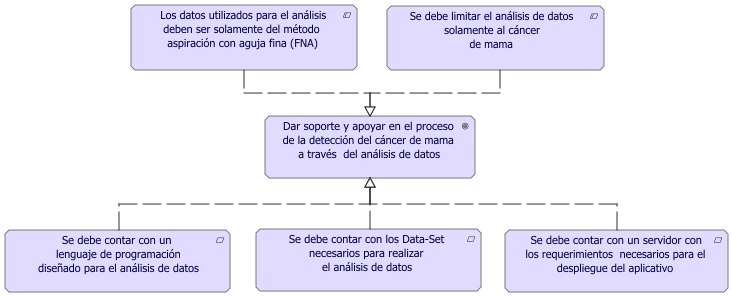
\includegraphics[width=1\linewidth]{ARQUITECTURA/imgs/CapaMotivacion/2_PvRealizacionObj}
	\caption{Punto de Vista de Realización de Objetivos}
	\label{PvRealizacionObj}
\end{figure}

\begin{enumerate}[label=\textbf{\arabic*})]
\item  \textbf{Dar soporte y apoyar en el proceso de la detección del cáncer de mama a través del análisis de datos:} el objetivo organizacional cuenta con tres requerimientos y dos restricciones. En este caso, este objetivo es el encargado de realizarlos.

\item  \textbf{Se debe contar con un lenguaje de programación diseñado para el análisis de datos:} Este requerimiento plantea que para poder generar el diagnostico de cáncer es necesario utilizar un lenguaje de programación que contenga herramientas y funcionalidades enfocados en el procesamiento y análisis de datos.

\item  \textbf{Se debe contar con los Data-Set necesarios para realizar el análisis de datos:} Este requerimiento se refiere a que los datos sobre los que se va a realizar el análisis deben contener variables de pacientes ya diagnosticados con cáncer de mama que permitan el entrenamiento de los algoritmos que clasificaran nuevos pacientes  candidatos de padecer dicho cáncer.

\newpage
\item  \textbf{Se debe contar con un servidor con los requerimientos necesarios para el despliegue del aplicativo:} Este requerimiento se refiere a que el servidor en el cual se va a desplegar el Back-End y el Front-End de la aplicación BreastApp debe contener las prestaciones de almacenamiento y procesamiento suficiente para la generación  optima de diagnósticos asociados al cáncer de mama.

\item  \textbf{Los datos utilizados para el análisis deben ser solamente del método aspiración con aguja fina (FNA):} Este restricción hace referencia a que las variables necesarias para el diagnostico de cáncer de mama deben ser solamente las obtenidas por el método FNA, esto debido a que el aplicativo esta diseñado para generar los diagnósticos con base solamente a este método.

\item  \textbf{Se debe limitar el análisis de datos solamente al cáncer de mama:} Este restricción hace referencia que el aplicativo esta enfocado solamente al cáncer de mama y no a otro tipo de cáncer. Se realiza esta limitación para que la generación de reportes sea rápida y el cáncer pueda tratarse a tiempo.
\end{enumerate}

%-------------Punto de Vista de Realización de Objetivos----------%
\newpage
\section{Punto de Vista de Contribución de Objetivos}

El Punto de Vista de Contribución de Objetivos permite a un analista modelar las relaciones de influencia entre objetivos y requisitos. Las vistas resultantes en este punto de vista pueden usarse para analizar el impacto que las metas tienen entre sí o para detectar conflictos entre los objetivos de las partes interesadas\cite{BolanosCastro2019}. 

En la Figura \ref{PvContribucionObj}, se plantea el Caso para el Punto de Vista de Contribución de Objetivos con cada uno de los elementos que interactúan entre sí. 

\begin{figure}[h!]
	\centering
	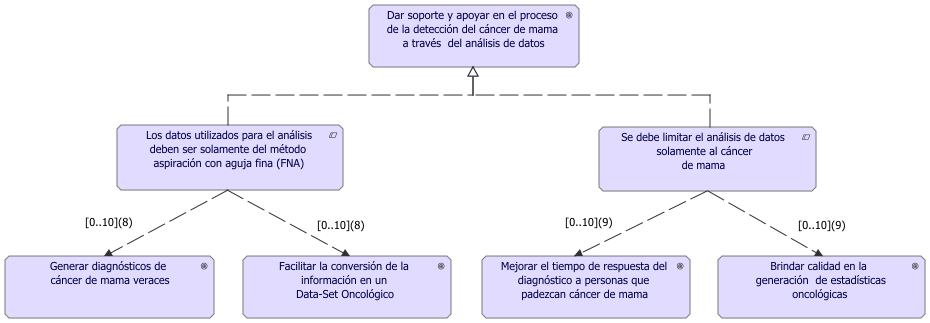
\includegraphics[width=1\linewidth]{ARQUITECTURA/imgs/CapaMotivacion/3_PvContribucionObj}
	\caption{Punto de Vista de Contribución de Objetivos}
	\label{PvContribucionObj}
\end{figure}

\begin{enumerate}[label=\textbf{\arabic*})]
	\item  \textbf{Dar soporte y apoyar en el proceso de la detección del cáncer de mama a través del análisis de datos:} para este punto de vista, se toman en cuenta las restricciones que realiza
	este objetivo organizacional, planteada en el modelo del punto de vista anterior. Esta se describe en el apartado siguiente.
	
	\item  \textbf{Los datos utilizados para el análisis deben ser solamente del método aspiración con aguja fina (FNA):} Este restricción hace referencia a que las variables necesarias para el diagnostico de cáncer de mama deben ser solamente las obtenidas por el método FNA, esto debido a que el aplicativo esta diseñado para generar los diagnósticos con base solamente a este método. Esta restricción tiene dos objetivos con impacto positivo. El impacto se mide en una escala de 1 a 10, siendo 10 el más alto y el impacto más positivo.
	
	\begin{itemize}
		\item  \textbf{\textit{Generar diagnósticos de cáncer de mama veraces:}} Teniendo en cuenta la restricción anterior se tiene un impacto positivo en este objetivo debido a que al procesar solamente datos obtenidos por el método de aguja fina(FNA) el entrenamiento de los algoritmos van a generar resultados cada vez mas precisos en la detección del cáncer de mama. El nivel de impacto asociado es de 8.
		
		\item  \textbf{\textit{Facilitar la conversión de la información en un Data-Set Oncológico:}}
		Teniendo en cuenta la restricción anterior se tiene un impacto positivo en este objetivo debido a que el método de aguja fina(FNA) es bastante utilizado en el ámbito medico,por lo que las estandarización e identificación de variables facilita la generación diversos Data-Set para el diagnostico de cáncer de mama.El nivel de impacto asociado es de 8.
	\end{itemize}
	
	\item  \textbf{Se debe limitar el análisis de datos solamente al cáncer de mama:} Este restricción hace referencia que el aplicativo esta enfocado solamente al cáncer de mama y no a otro tipo de cáncer. Se realiza esta limitación para que la generación de reportes sea rápida y el cáncer pueda tratarse a tiempo.Esta restricción tiene dos objetivos con impacto positivo. El impacto se mide en una escala de 1 a 10, siendo 10 el más alto y el impacto más positivo.
	
	\begin{itemize}
		\item  \textbf{\textit{Mejorar el tiempo de respuesta del diagnostico a personas que padecen cáncer de mama:}} Teniendo en cuenta la restricción anterior se tiene un impacto positivo debido a que al enfocarse solamente en el cáncer de mama la generación de diagnósticos es mas rápida ya que el sistema esta diseñado solamente para este tipo de cáncer.El nivel de impacto asociado es de 9.
		
		\item  \textbf{\textit{Brindar calidad en la generación de estadísticas Oncológicas:}} Teniendo en cuenta la restricción anterior se tiene un impacto positivo debido a que al enfocarse solamente en el cáncer de mama los algoritmos del sistema cada vez van a irse entrenando con una gran cantidad de datos mayor que va a garantizar cada vez un resultado mas exacto del diagnostico de cáncer de mama. 
	\end{itemize}

\end{enumerate}

%-------------Punto de Vista de Principios----------%
\newpage
\section{Punto de Vista de Principios}

El Punto de Vista de Principios permite al analista modelar los principios que son relevantes para el problema de diseño en cuestión, incluyendo los objetivos que motivan dichos principios \cite{BolanosCastro2019}. 

En la Figura \ref{PvPrincipios}, se plantea el Caso para el Punto de Vista de principios con cada uno de los elementos que interactúan entre sí. 

\begin{figure}[h!]
	\centering
	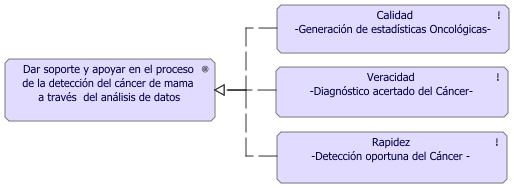
\includegraphics[width=1\linewidth]{ARQUITECTURA/imgs/CapaMotivacion/4_PvPrincipios}
	\caption{Punto de Vista de Principios}
	\label{PvPrincipios}
\end{figure}

\begin{enumerate}[label=\textbf{\arabic*})]
	\item  \textbf{Dar soporte y apoyar en el proceso de la detección del cáncer de mama a través del análisis de datos:} Este objetivo organizacional hace referencia a el servicio de generar diagnósticos relacionados con el cáncer de mama  solicitados por los diferentes funcionarios del Instituto de Cancerología.Realiza tres principios representativos para la organización, descritos a continuación.
	
	\begin{itemize}
		\item  \textbf{\textit{Calidad:}} Generación de estadísticas oncologicas con una adecuada organización para una mayor compresión y análisis.
		
		\item  \textbf{\textit{Veracidad:}} Precisión  alta en el diagnostico y detección del Cáncer de mama.
		
		\item  \textbf{\textit{Rapidez:}}  Generación de diagnósticos del cáncer de mama de forma eficiente para un tratamiento oportuno.
	\end{itemize}
\end{enumerate}

%-------------Punto de Vista Realización de Requerimientos----------%
\newpage
\section{Punto de Vista de Realización de Requerimientos }

El Punto de Vista de Realización de Requerimientos permite a los implicados modelar la realización de los requisitos por parte de los elementos básicos, como los actores empresariales y los servicios empresariales. Este punto de vista tiene en cuenta elementos como los procesos empresariales, los servicios y componentes de la aplicación. Además, puede usarse para refinar requisitos en requisitos mas detallados\cite{BolanosCastro2019}. 

En la Figura \ref{PvRealizacionReq}, se plantea el Caso para el Punto de Vista de Realización de Requerimientos con cada uno de los elementos que interactúan entre sí. 

\begin{figure}[h!]
	\centering
	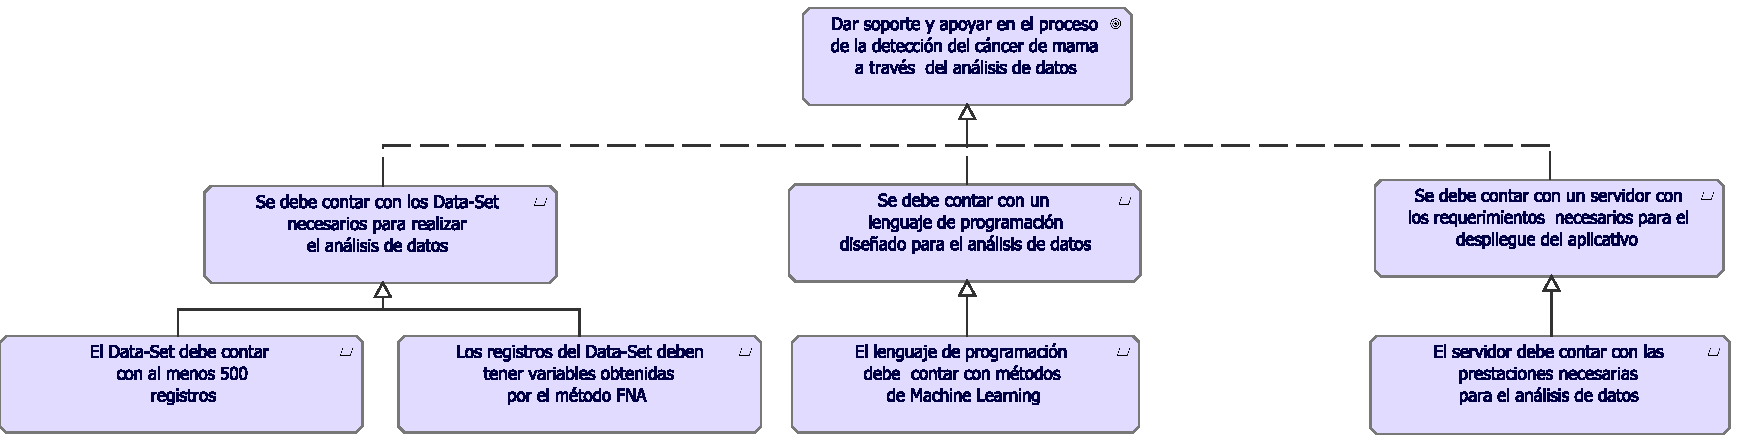
\includegraphics[width=1\linewidth]{ARQUITECTURA/imgs/CapaMotivacion/5_PvRealizacionReq}
	\caption{Punto de Vista de Realización de Requerimientos}
	\label{PvRealizacionReq}
\end{figure}

\begin{enumerate}[label=\textbf{\arabic*})]
	\item  \textbf{Dar soporte y apoyar en el proceso de la detección del cáncer de mama a través del análisis de datos:} El	objetivo organizacional cuenta con tres requerimientos. En este caso,
	este objetivo es el encargado de realizarlos.
	
	\item  \textbf{Se debe contar con un lenguaje de programación diseñado para el análisis de datos:} Este requerimiento plantea que para poder generar el diagnostico de cáncer es necesario utilizar un lenguaje de programación que contenga herramientas y funcionalidades enfocados en el procesamiento y análisis de datos. Este requerimiento tiene asociado los dos requerimientos que se detallan a continuación:
	
	\begin{itemize}
		\item  \textbf{\textit{El Data-Set debe contar con al menos 500 registros:}} Es necesario para el entrenamiento de los algoritmos de Machine Learning contar con información mayor o igual a 500 registros de pacientes los cuales incluyan las variables necesarias para el entrenamiento de dichos algoritmos para realizar posteriormente el diagnostico de nuevos pacientes.   
		
		\item  \textbf{\textit{Los registros del Data-Set deben tener variables obtenidas por el método FNA:}} Es necesario que las variables obtenidas sean del método medico de  aspiración con aguja fina (FNA) esto debido a que el aplicativo esta diseñado para generar los diagnósticos con base solamente a este método.
	\end{itemize}
	
	\item  \textbf{Se debe contar con un lenguaje de programación diseñado para el análisis de datos:} Este requerimiento plantea que para poder generar que el diagnostico de cáncer es necesario utilizar un lenguaje de programación que contenga herramientas y funcionalidades enfocados en el procesamiento y análisis de datos. Este requerimiento tiene asociado el requerimiento que se detalla a continuación:
	
	\begin{itemize}
		\item  \textbf{\textit{El lenguaje de programación debe contar con métodos de Machine Learning:}} Es necesario que el lenguaje de programación cuente con métodos de Machine Learning debido a que por medio de ellos es que se realiza el diagnostico de cáncer de mama.
	\end{itemize}
	
	\item  \textbf{Se debe contar con un servidor con los requerimientos necesarios para el despliegue del aplicativo:} Este requerimiento se refiere a que el servidor en el cual se va a desplegar el Back-End y el Front-End de la aplicación BreastApp debe contener las prestaciones de almacenamiento y procesamiento suficiente para la generación  optima de diagnósticos asociados al cáncer de mama. Este requerimiento tiene asociado el requerimiento que se detalla a continuación:
	
	\begin{itemize}
		\item  \textbf{\textit{El servidor debe contar con las	prestaciones necesarias para el análisis de datos:}} Es necesario que el servidor cuente con la memoria suficiente de almacenamiento y procesamiento  debido a que la cantidad de datos y cálculos realizados por los métodos de Machine Learning es bastante alta.
	\end{itemize}
	
\end{enumerate}

%-------------Punto de Vista de Motivación----------%
\newpage
\section{Punto de Vista de Motivación }

El Punto de Vista de Motivación permite al diseñador o analista modelar el aspecto de las razones (motivaciones), que guían el diseño o el cambio de una Arquitectura Empresarial.Este punto de vista puede utilizarse para presentar un panorama completo o parcial del aspecto de la motivación relacionando a las
partes interesadas, sus objetivos principales, los principios que se aplican y los principales requisitos de servicios, procesos, aplicaciones y objetos\cite{BolanosCastro2019}. 

En la Figura \ref{PvMotivacion}, se plantea el Caso para el Punto de Vista de Motivación con cada uno de los elementos que interactúan entre sí. 

\begin{figure}[h!]
	\centering
	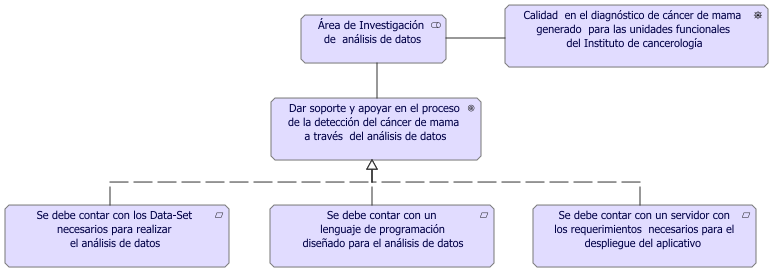
\includegraphics[width=1\linewidth]{ARQUITECTURA/imgs/CapaMotivacion/6_PvMotivacion}
	\caption{Punto de Vista de Motivación}
	\label{PvMotivacion}
\end{figure}

\begin{enumerate}[label=\textbf{\arabic*})]
	\item  \textbf{Dar soporte y apoyar en el proceso de la detección del cáncer de mama a través del análisis de datos:} El objetivo organizacional cuenta con tres requerimientos. En este caso, este objetivo es el encargado de realizarlos. Ademas, se asocia con el StakeHolder \textit{Área de Investigación de  análisis de datos}.
	
	\item  \textbf{Se debe contar con un lenguaje de programación diseñado para el análisis de datos:} Este requerimiento plantea que para poder generar el diagnostico de cáncer es necesario utilizar un lenguaje de programación que contenga herramientas y funcionalidades enfocados en el procesamiento y análisis de datos.
	
	\item  \textbf{Se debe contar con los Data-Set necesarios para realizar el análisis de datos:} Este requerimiento se refiere a que los datos sobre los que se va a realizar el análisis deben contener variables de pacientes ya diagnosticados con cáncer de mama que permitan el entrenamiento de los algoritmos que clasificaran nuevos pacientes  candidatos de padecer dicho cáncer.
	
	\item  \textbf{Se debe contar con un servidor con los requerimientos necesarios para el despliegue del aplicativo:} Este requerimiento se refiere a que el servidor en el cual se va a desplegar el Back-End y el Front-End de la aplicación BreastApp debe contener las prestaciones de almacenamiento y procesamiento suficiente para la generación  optima de diagnósticos asociados al cáncer de mama.

	\item  \textbf{Calidad  en el diagnóstico de cáncer de mama generado para las unidades funcionales del Instituto de cancerología:} Este conductor hace referencia a la búsqueda de mejoramiento en la atención a pacientes de los investigadores de la Subdirección de Investigaciones, otras Subdirecciones y demás unidades funcionales del Instituto de Cancerología con base en la generación de diagnosticos de cáncer de mama con un nivel de calidad alto .Se asocia con el StakeHolder \textit{Área de Investigación de análisis de datos}.	
\end{enumerate}


